%Dokumentinnstillinger:---------------------------------
%Ved å google flitting kan du finne ut hva de forskjellige tingene her betyr, og hvordan du kan gjøre eventuelle endringer.
\documentclass[a4paper,11pt,norsk]{article}
\usepackage[utf8]{inputenc}
\usepackage{a4wide}
\usepackage{lmodern}
\usepackage[T1]{fontenc}
\usepackage{babel}

\setlength{\parindent}{0pt} 
\setlength{\parskip}{2ex}
\usepackage{fixltx2e}
\usepackage{amsmath}
\usepackage[pdftex, pdfborderstyle={/S/U/W 0}]{hyperref}
\usepackage{graphicx}
\usepackage[font=small,labelfont=bf]{caption}
\usepackage{tabularx}
\usepackage{multirow}
\usepackage{circuitikz}
\usepackage{pst-node,pst-circ}
% Adds seperation between two elements with a comma. Format: "    ,    ".
\newcommand{\comma}{\quad , \quad}
% Gives double underline under selected text.
\def\dunderline#1{\underline{\underline{#1}}}
% Faster way to make an equation that can be formatted with "&" to look nice.
\def\spliteq#1{\begin{equation}\begin{split}{#1}\end{split}\end{equation}\\}
%------------------------------------- End -------------------------------------

\begin{document}

%Headingdel:---------------------------------------------
\begin{minipage}[c]{0.15\textwidth}

\includegraphics[width=2.0cm]{elsys_pos_staaende_ntnu.png}
\end{minipage}
\begin{minipage}[c]{0.85\textwidth}

\renewcommand{\arraystretch}{1.7}
\large 
\begin{tabularx}{\textwidth}{|X|X|}
\hline
\multicolumn{2}{|l|}{} \\
\multicolumn{2}{|l|}{\huge \textbf{Designnotat 5}} \\
\multicolumn{2}{|l|}{}  \\
\hline
\multicolumn{2}{|l|}{Tittel: 
%Skriv inn tittel her:------------------------------------------
Emitter-følger (diskréte buffer)
} \\
\hline
\multicolumn{2}{|l|}{Forfattere: 
%Skriv inn forfattere her:--------------------------------------
Sindre Danielsen
} \\
\hline
%Skriv inn versjon og dato her her:-----------------------------
Versjon: 1.1 & Dato: 31.10.21
\\
\hline 
\end{tabularx}
\end{minipage}
\normalsize

%Automatisk generert innholdsfortegnelse:------------------

\setlength{\parskip}{0ex}
\renewcommand{\baselinestretch}{0.1}\normalsize
\tableofcontents
\renewcommand{\baselinestretch}{1.00}\normalsize
\setlength{\parskip}{2ex}
\rule{\textwidth}{1pt}

%Selve rapporten:----------------------------------------÷
\newpage
\section{Problembeskrivelse}
\label{sec:innledning}
Når en krets inneholder flere delsystemer eller komponenter, så er det ofte uønsket at de skal oppføre seg som spenning-/strøm delere. Det kan da brukes en buffer eventuelt før og etter slike delsystemer. I de tilfeller er op-amper vanlig å bruke (spenningsfølger) \cite{buffer_article}.
\\\\
Når op-amper ikke er tilgjengelige, eller ikke har ønskede egenskaper, som båndbredde og effekt. Da kan diskréte komponenter, som transistorer, kondensatorer og motstander brukes. Designnotatet vil gå gjennom en løsning på hvordan en diskréte buffer kan utvikles. \\
Et generelt bufferoppsett er vist ved figur~\ref{fig: generell bufferkrets}. \\
\begin{figure}[htbp]
    \centering
    \begin{circuitikz} [american voltages, european resistors, baseline=(current bounding box.center)]
        \ctikzset { label/align = straight }
        \draw (0,2)
        to [V, l=$V_0$] (0,0);
        
        \draw (0,2)
        % Top-left side
        to[R=$R_{k}$] (2.5,2)
        to[short,i=$i$, -o] (4,2)
        node[above] {$v_i$}
        to[short] (4.5,2);
        
        % Op amp
        \draw (4,2) ++ (1,0) node[buffer]
        % Top-right side
        (buffer.out) ++ (0.5,0) to[short,-o] ++ (0.5,0)
        node[above] {$v_o$}
        to[short] ++ (2,0)
        to[R=$R_L$] ++ (0, -2);
        
                \draw (0,0)         
                % Kilde text        
                (0,-0.9) node[below] {Kilde}         
                % Last text         
                (7.5,-0.9) node[below] {Last};
        
        % Ground Source
        \draw (0,0) to (0,0) node[ground]{}; 
        % Ground Load
        \draw (8,0) to (8,0) node[ground]{};
        % Left dashed box
        \node[draw,dashed,minimum width=3.2cm,minimum height=3.8cm,anchor=south west] at (-0.75,-0.90)
        ;
        % Right dashed box
        \node[draw,dashed,minimum width=2.5cm,minimum height=3.8cm,anchor=south west] at (7,-0.90);

        
    \end{circuitikz}
    \caption{En buffer mellom to delsystemer.}
  \label{fig: generell bufferkrets}
\end{figure}
\\
Figuren består av en spenningskilde $V_0$ med en kildemotstand $R_k$, en inngangsstrøm $i$ på bufferen og en lastmostand $R_L$. Definerer bufferen som trekanten mellom $v_i$ og $v_o$.
\\\\
En god buffer har følgende kriterier:
\begin{itemize}
    \item Forholdet mellom amplituden på utgangssignalet $v_o$ og inngangssignalet $v_i$: \\ $\frac{A_o}{A_i} \rightarrow 1$, der $A_o$ og $A_i$ er amplituden på respektivt $v_o$ og $v_i$.
    \item Ingen klipping på $v_o$.
    \item Høy inngangsimpedans og lav utgangsimpedans.
    \item Knekkfrekvens ved -3dB i frekvensdomene.
\end{itemize}

\newpage
\section{Prinsipiell løsning}
\label{sec:prinsipielllosning}
Det interessante er det som foregår inni bufferen. I figur~\ref{fig: emitter-følger} er det satt opp et kretsskjema over bufferen sitt innhold.
\\
\begin{figure}[htbp]
    \centering
    \begin{circuitikz} [american voltages, european resistors, european vresistors, baseline=(current bounding box.center)]
        \ctikzset { label/align = straight }
        \coordinate (R_2) at (2,0);
        \coordinate (V_B) at (2,4);
        \coordinate (R_E) at (4,0);
        \coordinate (V_CC_i) at (2, 8);
        \coordinate (V_CC_o) at (8, 8);
        
        \draw 
        % Ground
        (R_2) ++ (R_2) ++ (R_2) to[short, o-o] (0,0)
        % Source V_CC
        (V_B) ++ (V_B) ++ (-4,0) to[short, l=$V_{CC}$] ++ (6,0)
        (V_B) to[short, R=$R_2$] (R_2)
        (V_B) to[short, C=$C_1$,o-o] ++ (-2,0)
        (V_B) ++ (V_B) ++ (-2, 0) to[short, R=$R_1$] (V_B)
        (V_B) ++ (2,0) node[npn] (npn) {}
        (npn.B) [short,-*] -- (V_B)
        (V_B) ++ (V_B) to[short] (npn.C)
        (npn.E) to[short, R=$R_E$, o-] (R_E)
        (npn.E) to[C=$C_2$, -o] ++ (2, 0);
        \draw
        % v_i
        (0, 3) to[open, v=$v_i(t)$] (0,1)
        %v_o
        (6, 2.5) to[open, v=$v_o(t)$] (6,0.5)
        ;
        
        \node[ground] (ground) at (3, 0) {};
       \node[] at (2.4,4.4) {$V_B$};
        
        
    \end{circuitikz}
    \caption{En variant av bufferen kalt en emitter-følger.}
    \label{fig: emitter-følger}
\end{figure} \\
Kretsen viser en buffer, som ikke inverterer signalet. Den mangler feedback egenskapen som en op-amp har. Det vil si at databladet til transistoren i kretsen er nødvendig for å utvikle systemet, siden strøm og spenning over transistoren bestemmer egenskapene til den.
\\\newpage
\subsection{Fjerne DC-bias} \label{subsec: DC-bias}
Kondensatorene $C_1$ og $C_2$ brukes for å fjerne DC-bias.
De har stor kapasitans, som gir en høy impedans for lave frekvenser. Enhver DC-bias på $v_i(t)$ vil da ikke forstyrre bufferen, samt at spenningskilden $V_{CC}$ vil ikke forstyrre utgangssignalet $v_o(t)$. Definerer frekvensen $f_{min}$ som den minste frekvensen uten kortslutning (knekkfrekvensen). Vi kan finne den ønskede kapasitansen for kondensatoren ved å isolere kapasitansen $C$ i likningen for et høypass filter:
\begin{equation} \label{eq: C_1}
    C_1 = \frac{1}{2\pi f_{min} \cdot Z_i}
\end{equation}
og
\begin{equation} \label{eq: C_2}
    C_2 = \frac{1}{2\pi f_{min} \cdot Z_o} \: .
\end{equation}
\\
Her er henholdsvis $Z_i$ og $Z_o$ inngangs- og utgangsimpedansen. 
\newpage
\subsection{Regulere klipping av signalet}
\label{subsec: klipping}
For å få bedre kontroll over klipping av signalet, så burde arbeidspunktet $V_B$ bestemmes nøye. Et anbefalt arbeidsområdet burde ligge midt mellom DC-kilden $V_{CC}$ og potensialet fra basen til emitter av transistoren $V_{BE}$: \\
\begin{equation} \label{eq: V_B}
    V_B = \frac{V_{CC} + V_{BE}}{2}.
\end{equation} \\
Grafisk vises det ved figur~\ref{fig: V_B}.
\begin{figure}[htbp]
    \centering
    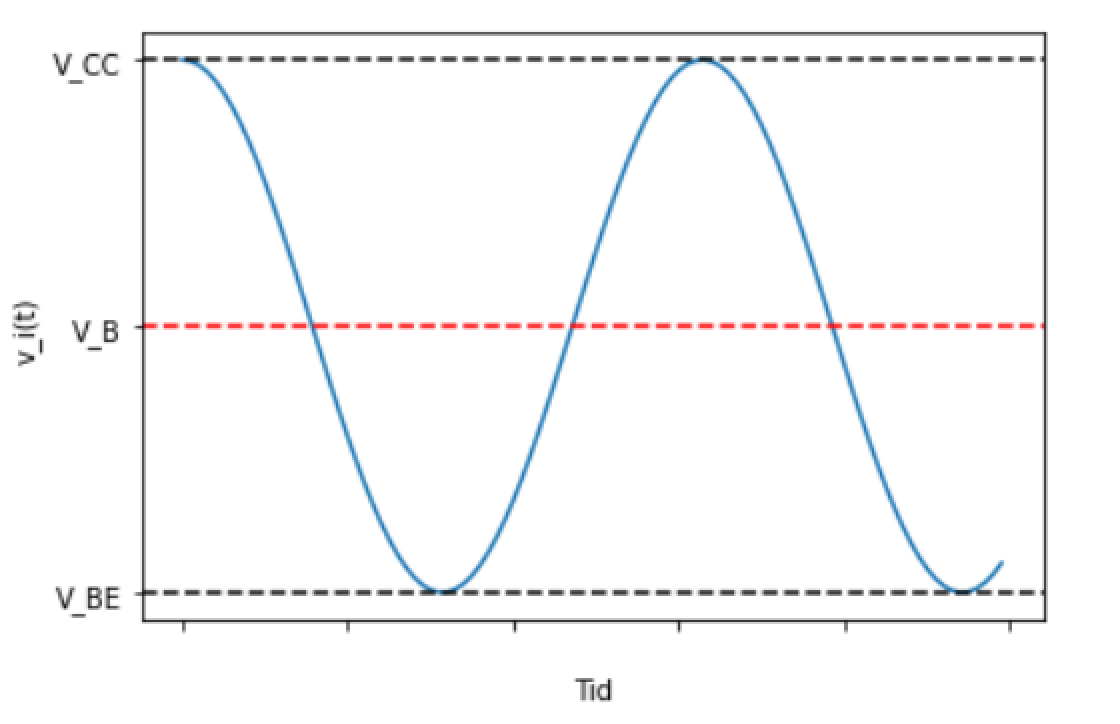
\includegraphics[width=1.0\textwidth]{img/Arbeidspunktet.png}
    \caption{Sentrerer klipping på $v_i(t)$ rundt $V_B$.}
    \label{fig: V_B}
\end{figure} \\
Hvis $v_i(t) > V_{CC}$ eller $v_i(t) < V_{BE}$, så vil signalet klippes.
\newpage
\subsection{Utvikle arbeidspunktet}
\label{subsec: rekne arbeidspunkt}
For å utvikle arbeidspunktet i seksjon~\ref{subsec: klipping}, så bestemmes $R_1$ og $R_2$ ved spenningsdelingen for $V_B$:
\begin{equation} \label{eq: R_1}
    R_1 = R_2 \left(\frac{V_{CC}}{V_B} - 1\right)
\end{equation}
Slik at her kan en motstand velges og den andre kan reknes ut. 
\\\\
Seksjon~\ref{subsec: bestemme R_E} viser at $i_b$ er bestemt av $R_E$.
En av karakteristikkene til transistoren er $\beta$ (ofte kalt $h_{FE}$ i datablad):
\begin{equation} \label{eq: beta}
    \beta = \frac{i_c}{i_b}.
\end{equation}
Den ønskes ofte å være i et område der $h_{FE}$ ikke endrer seg ved $i_c$, se eksempelet i figur~\ref{fig: h_FE-i_C kurve}. \\
\begin{figure}[htbp]
    \centering
    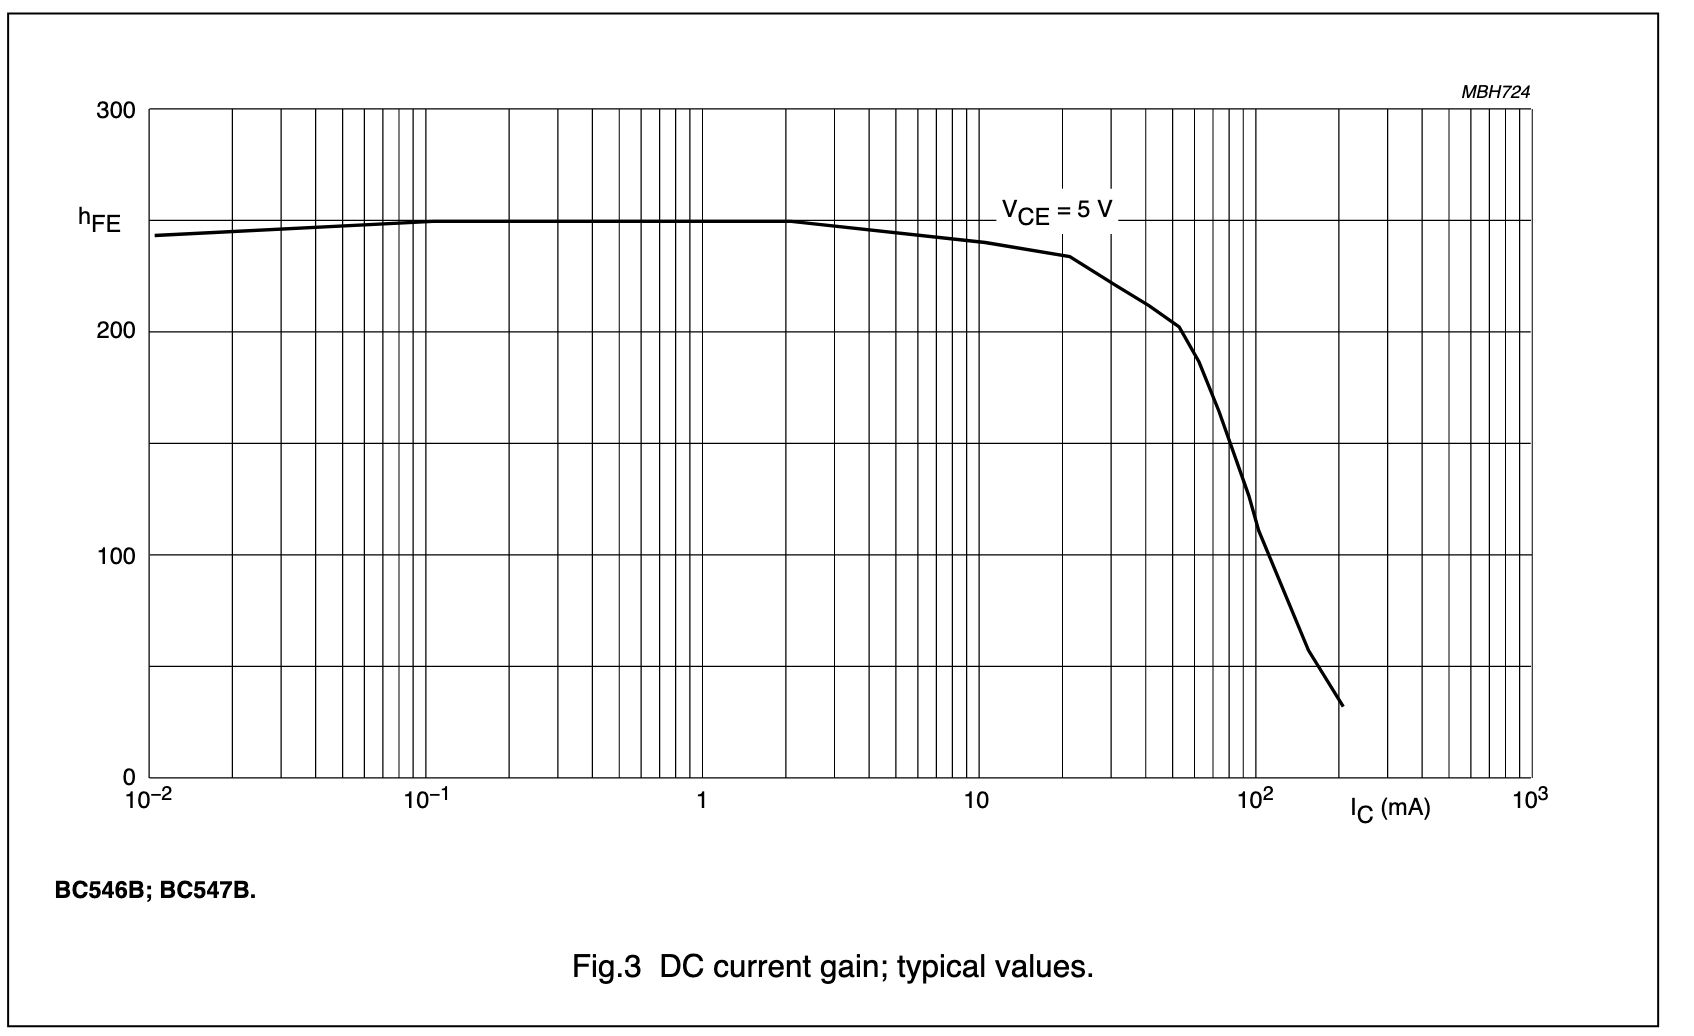
\includegraphics[width=1.0\textwidth]{img/h_FE-I_C kurve.png}
    \caption{Eksempel på hvordan $\beta$ ($h_{FE}$) varierer med $i_C$ \cite{BC547B Datasheet}.}
    \label{fig: h_FE-i_C kurve}
\end{figure} \\
Slik vi ser her, så burde $i_C \leq 2$mA. \\
Databladet forteller også maksimalverdien til $i_C$, som ikke burde overskrides.
\newpage
\subsubsection{Bestemme $R_E$}\label{subsec: bestemme R_E}
Vi kan bestemme $R_E$ ved å velge $i_b$. KVL for arbeidspunktet og Ohms lov for $R_E$ gir de to følgende likningene:
\begin{equation} \label{eq: V_E}
    V_E = V_B - V_{BE}
\end{equation}\\
og
\begin{equation} \label{eq: i_e}
    i_e = \frac{V_E}{R_E} \: , \quad \quad \textrm{der} \quad i_e = (1+\beta)i_b \: .
\end{equation}\\
Ved å løse for likning~\ref{eq: i_e} og å isolere $R_E$ får vi at:
\begin{equation} \label{eq: R_E}
    R_E = \frac{V_B - V_{BE}}{i_b(\beta +1)} \: .
\end{equation}



\newpage
\subsection{Småsignalmodellen}
Generelt for en buffer, så ønskes inngangsimpedansen $Z_i \rightarrow \infty$ og utgangsimpedansen $Z_o \rightarrow 0$. Dette gjelder ikke alltid for emitter-følgere, på grunn av at hvis $R_1, R_2$ eller $R_E$ øker, så vil $i_b$ også øke. Transistorene har en maksimalgrense på $i_c$, som definert i databladet. 

Ved å bruke en småsignalmodell vist i figur~\ref{fig: småsignalmodell}, så kan vi enklere utvikle uttrykk for $Z_i$ og $Z_o$. 
\\
\begin{figure}[htbp]
    \centering
    \begin{circuitikz} [american voltages, american currents, european resistors, european vresistors, baseline=(current bounding box.center)]
        \ctikzset { label/align = straight }
        \coordinate (R_1) at (1,0);
        \coordinate (R_2) at (3,0);
        \coordinate (B) at (4,4);
        \coordinate (iC) at (6,0);
        \coordinate (R_E) at (10,0);
        \coordinate (v_i) at (0, 4);
        \coordinate (v_o) at (11,4);
        \coordinate (E) at (7,2);
        
        \draw 
        % Ground
        (v_o) ++ (0,-4) to[short, o-o] (0,0)
        % v_i
        (v_i) to[short, o-o] (B)
        % R_1
        (v_i) ++ (1,0) to[short, R=$R_1$] (R_1)
        % R_2
        (v_i) ++ (3,0) to[short, R=$R_2$] (R_2)
        % i_b
        (B) ++ (-1,0) to[short, i=$i_b$] ++ (0.5,0)
        % Basen
        (B) ++ (0,0.3) node[] {$B$}
        %r_pi
        (B) ++ (2,0) to[short, R=$r_{\pi}$] (B)
        % Til styrte strømkilden
        (iC)
        to[cI, -o] ++ (0,4)
        % Til v_o
        to[short, -o] (v_o)
        % i_e
        (iC) ++ (2,4) to[short, i=$i_e\textit{ = } (1+\beta)i_b$] ++ (2,0)
        % Til R_E
        (R_E) to[short, R=$R_E$] ++ (0, 4)
        % Controlled current source label
        (iC) ++ (1,2) node[] {$\beta \: i_b$}
        % Collector
        (iC) to[short, -o] ++(0,1)
        % Collector label
        (iC) ++ (0.3,1) node[] {$C$}
        % Emitter
        (iC) ++ (1,4) to[short, -o] ++ (0,0)
        % Emitter label
        (iC) ++ (1,4.4) node[] {$E$}
        % Spenningskilde
        (0,0) -- (-2,0)
        to[V, v=$V_0$, invert] ++ (0, 4)
        to[short, R=$R_k$] (v_i)
        
        % Lastmotstand
        (v_o) to[short] ++ (1,0)
        to[short, R=$R_L$] ++(0,-4)
        -- ++ (-1,0)
        ;
        \draw
        % v_i
        (0, 3) to[open, v=$v_i(t)$] (0,1)
        % v_o
        (11, 3) to[open, v=$v_o(t)$] (11,1);
        \node[ground] (ground) at (3, 0) {};
        
        
    \end{circuitikz}
    \caption{Småsignalmodell av figur~\ref{fig: emitter-følger} koblet på spenningskilde og lastmotstand.}
    \label{fig: småsignalmodell}
\end{figure} \\
Legg merke til at $R_1$ og $R_2$ er i parallell, så vi definerer det som $R_B$. Vi definerer også $R_{o}$ som parallelen av $R_E$ og $R_L$. På likningsform har vi
\begin{equation} \label{eq: R_B}
    R_B = R_1 || R_2 = \frac{1}{\frac{1}{R_1} + \frac{1}{R_2}}
\end{equation}
og
\begin{equation} \label{eq: R_o}
    R_o = R_E || R_L = \frac{1}{\frac{1}{R_E} + \frac{1}{R_L}} \: .
\end{equation}
\\\\
Motstanden fra basen til emitter er gitt ved:
\begin{equation} \label{eq: r_{pi}}
    r_\pi = \frac{\beta V_T}{I_C} \: ,
\end{equation}\\
der den termiske spenningen $V_T \approx 26$mV ved romtemperatur. Den endres litt avhengig av temperaturen \cite{Thermal Voltage}.
\newpage

\subsubsection{Spenningsforsterkning}
Spenningsforsterkningen er gitt ved $A_v = \frac{v_o}{v_i}$. \\\\
Vi har $v_o$ gitt ved ohms lov:
\begin{equation} \label{eq: v_o}
    v_o = R_o \cdot i_e = R_o\cdot(1+\beta)i_b
\end{equation}
og $v_i$ ved bruk av $i_b$ og KVL:
\begin{equation}\label{eq: v_i} \label{eq: v_i}
    v_i = i_b\left(r_\pi + (1+\beta) \cdot R_o \right)\:.
\end{equation}
\\\\
Emitter-følgeren vil da gi en spenningsforsterkning
\begin{equation} \label{eq: A_v}
    A_v = \frac{(1+\beta)R_o}{r_\pi + (1+\beta)R_o} \:.
\end{equation}
Fra uttrykket ser vi $A_v$ nærmer seg 1, men den vil alltid avvike litt på grunn av transistorens motstand $r_\pi$. Merk også at $A_v$ er positiv, som stemmer med $v_o$ på figur~\ref{fig: emitter-følger}. Den viser at at $v_o$ følger $v_i$, derfor navnet emitter-følger.


\subsubsection{Inngangsimpedansen}
\label{subsec: inngangsimpedans}
Inngangsimpedansen $Z_i$ er gitt ved
\begin{equation} \label{eq: Z_i}
    Z_i = R_B || Z_{ii} = \frac{1}{\frac{1}{R_B} + \frac{1}{Z_{ii}}}.
\end{equation}
der inngangsimpedansen $Z_{ii}$ er impedansen vi får når vi ser inn på basen av transistoren. Det oppnår vi ved å dele $v_i$ på $i_b$. Likning \ref{eq: v_i} gir at
\begin{equation} \label{eq: Z_{ii}}
    Z_{ii} = \frac{v_i}{i_b} = r_\pi + (1+\beta)R_o \:.
\end{equation}


\newpage

\subsubsection{Utgangsimpedansen}
\label{subsec: utgangsimpedans}
For å finne utgangsimpedansen, så kreves et par endringer på figur~\ref{fig: småsignalmodell}.
\begin{itemize}
    \item Skru av kilden til signalet.
    \item Erstatt $R_L$ med en testkilde $v_x$ (spenning), som har en teststrøm $i_x$.
\end{itemize}
Utgangsimpedansen er gitt fra
\begin{equation} \label{eq: Z_o first}
    Z_o = \frac{v_x}{i_x}
\end{equation}\\
For å finne forholdet mellom $v_x$ og $i_x$, så må vi bruke to likning som involverer begge. \\Eksempelvis summere strømmene over $R_E$, som gjøres ved
\begin{equation}\label{eq: utgangsimpedans med x}
    i_e + i_x = \frac{v_x}{R_E} \quad \implies \quad i_b + \beta i_b + i_x = \frac{v_x}{R_E} \: .
\end{equation}\\
Siden det er to ukjente, så trenger vi en likning til. Vi kan bruke KVL, som gir at:
\begin{equation} \label{eq: utgangsimpedans 2 med x}
    v_x + r_\pi i_b + R_i i_b = 0 \:,
\end{equation}\\
der
\begin{equation} \label{eq: R_i}
    R_i = \frac{1}{\frac{1}{R_k} + \frac{1}{R_1} + \frac{1}{R_2}} \: .
\end{equation}
\\\\
Ved å løse for $i_b$ og substituere inn i likning~\ref{eq: utgangsimpedans med x}, så får vi:
\begin{equation} \label{eq: Z_o final}
    Z_o = \frac{1}{\frac{1+\beta}{R_i+r_\pi} + \frac{1}{R_E}} \: .
\end{equation}

\newpage

\newpage
\section{Realisering og test}
\label{sec:realisering}
Oppkoblingen av kretsen bruker komponentverdiene gitt ved tabell~\ref{table: reelle verdier}.
\begin{table}[htbp]
\centering
\begin{tabular}{ |c|c|c|c| } 
\hline
\textbf{Navn} & \textbf{Verdi}\\
\hline
$R_k$ & $1$k$\Omega$.
\\
\hline
$R_L$ & $179.9\Omega$
\\
\hline
$V_{CC}$ & $9$V
\\
\hline
$R_E$ & $2.1$k$\Omega$ \\
\hline
$R_2$ & $199.7$k$\Omega$
\\
\hline
$R_1$ & $171$k$\Omega$.
\\
\hline
$C_1$ & $324$nF
\\
\hline
$C_2$ & $200\mu$F
\\
\hline
\end{tabular}
\caption{Reelle verdier basert på tabell~\ref{table: komponenter}.}
\label{table: reelle verdier}
\end{table}
\\
\begin{table}[htbp]
\centering
\begin{tabular}{ |c|c|c|c| } 
\hline
\textbf{Navn} & \textbf{Verdi} & \textbf{Beskrivelse}\\
\hline

\hline
$R_k$ & $1$k$\Omega$ & Valgt motstand på AC-kilden.
\\
\hline
$R_L$ & $180\Omega$ & Valgt motstand på lasten.
\\
\hline
$V_{CC}$ & $9$V & DC-kilden til bufferen.
\\
\hline
$V_0$ & $A_0 sin(f_0 t)$  & AC-kilden.
\\
\hline
$R_E$ & $2.1$k$\Omega$ & Likning~\ref{eq: R_E}. \\
\hline
$R_2$ & $200$k$\Omega$ & Velgt motstandsverdi.
\\
\hline
$R_1$ & $171.1$k$\Omega$ & Likning~\ref{eq: R_1}.
\\
\hline
$C_1$ & $311.2$nF & Likning~\ref{eq: C_1}.
\\
\hline
$C_2$ & $191.2\mu$F & Likning~\ref{eq: C_2}.
\\
\hline
~ & BC547B & Transistor modell, datablad: \cite{BC547B Datasheet}. \\
\hline
\end{tabular}
\caption{Teoretiske komponentverdier}
\label{table: komponenter}
\end{table}

\newpage

\begin{table}[htbp]
\centering
\begin{tabular}{ |c|c|c|c| } 
\hline
\textbf{Navn} & \textbf{Verdi} & \textbf{Beskrivelse}\\
\hline
$f_0$ & $1000$Hz & Valgt frekvens påkoblet $v_i(t)$.\\
\hline
$A_0$ & $500$mV & Valgt amplitude på $v_i(t)$.\\
\hline
$i_C$ & $2$mA & Velger en ønsket collector strøm i systemet, som gjør datablad enkelt i bruk. \\
\hline
$V_{BE}$ & $700$mV & Base-emitter metningsspenning (Se figur~\ref{fig: base-emitter on voltage}). \\
& & Egentlig verdi $\approx 660$mV. Brukte litt større i utrekning for å få $V_B$ hevet litt. \\
& & Tar da i betrakning små uforventede spenningsfall, som kan klippe signalet. \\
\hline
$f_{min}$ & $25$Hz & Valgt knekkfrekvens, grunnet bregrenset med kondensatorer.
\\
\hline
$\beta$ & $290$ & Typisk $h_{FE}$ i databladet. \cite{BC547B Datasheet}.
\\
\hline
$r_{\pi}$ & $3,8$k$\Omega$ & Likning~\ref{eq: r_{pi}}.
\\
\hline
$V_B$ & $4.85$V & Likning~\ref{eq: V_B}.
\\
\hline
$R_B$ & $92.2$k$\Omega$ & Likning~\ref{eq: R_B}.
\\
\hline
$R_o$ & $165.6\Omega$ & Likning~\ref{eq: R_o}.
\\
\hline
$A_v$ & $0.927$ & Likning~\ref{eq: A_v}. \\
\hline
$Z_i$ & $33.2$k$\Omega$ & Likning~\ref{eq: Z_i}.
\\
\hline
$Z_o$ & $16.2\Omega$  & Likning~\ref{eq: Z_o final}.
\\
\hline
\end{tabular}
\caption{Teoretiske verdier for variablene.}
\label{table: variabler}
\end{table}
\\
\begin{figure}[htbp]
    \centering
    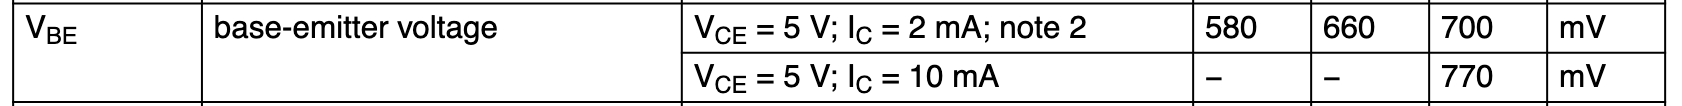
\includegraphics[width=1.0\textwidth]{img/Base-emitter on voltage.png}
    \caption{$V_{BE}$ for BC547B, Min.: $580$mV, Typisk: $660$mV, Maks.: $700$mV  \cite{BC547B Datasheet}.}
    \label{fig: base-emitter on voltage}
\end{figure}\\
Kondensator-verdiene vil være litt større enn fra de teoretiske pga. av begrenset tilgang til serie-/parallell koblinger. Når man gjør de større så vil $f_{min}$ bli litt mindre, se likning~\ref{eq: C_1}. \\

Merk at: Siden $C_1$ eller $C_2$ er større enn $1\mu$F, så kan det være gunstig å bruke to polare elektrolytte kondensatorer i  $\textit{reversert seriekobling}$ for å skape kapasitans. Det vil si at den første kondensatoren har den positive polen som inngang, og den andre kondensatoren har positiv pol som utgang. Årsaken bak dette er at ikke-polare kondensatorer har som regel ikke så stor kapasitans, som ønsket.
Her må begge kondensatorene ha lik kapasitans og maksimal spenning. På den måten unngåes problemer med spenningspotensialet fra positiv til negativ pol, som kan bli et problem over tid når det brukes AC spenning.
De vil følge samme regler som vanlig seriekobling, der kapasitansen halveres ved reversert seriekobling.

\newpage
\subsection{Første resultat}
Signalanalyse av spenning over tid for $v_i(t)$ og $v_o(t)$ vises ved figur~\ref{fig: initial signal}. \\
\begin{figure}[htbp]
    \centering
    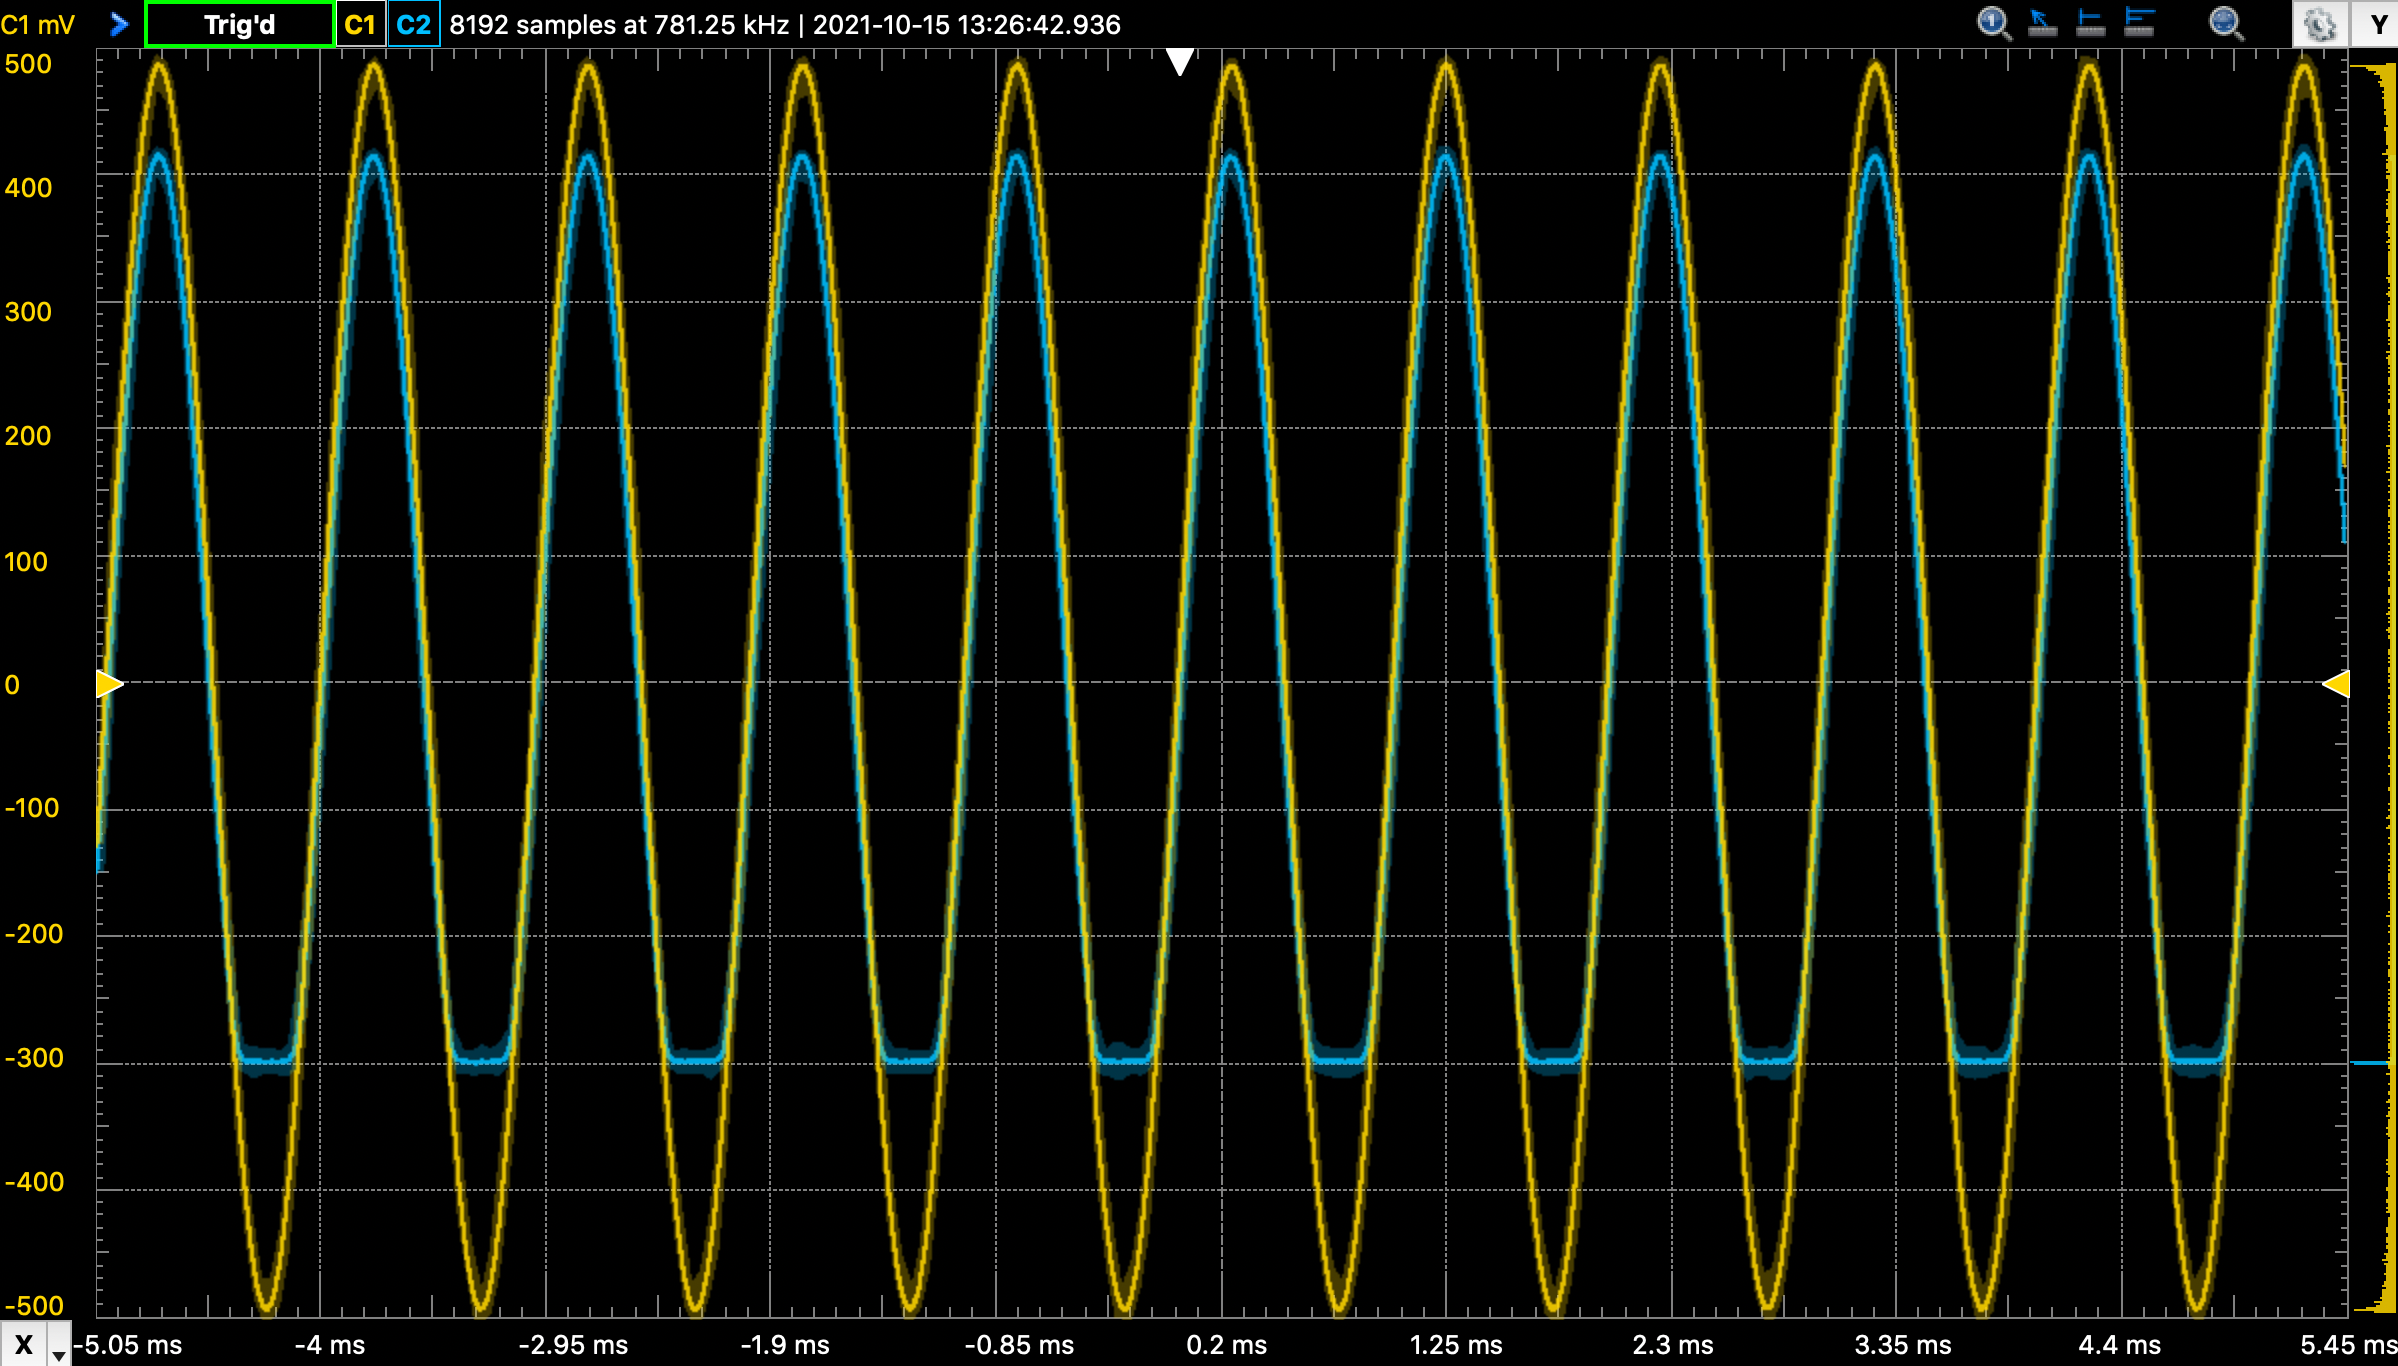
\includegraphics[width=1.0\textwidth]{img/Initial signal.png}
    \caption{Realisert modell: [V/t] der Gul: $v_i(t)$ og Turkis: $v_o(t)$.}
    \label{fig: initial signal}
\end{figure}\\
Klipping foregår ved $v_o=-300$mV, som betyr at $V_B$ er for lav, slik forklart i seksjon~\ref{subsec: klipping}. På grunn av den betydelige forstyrrelse i $v_o(t)$, så velges det å endre på $V_B$ før noe annet diskuteres.
Det gjøres ved å justere på $R_1$ eller $R_2$, se likning~\ref{eq: R_1}. I seksjon~\ref{subsec: improved signal} endres $R_1$ slik at vi får et signal som kan jobbes med.

\newpage

Den oppkoblede kretsen er vist ved figur~\ref{fig: first circuit}.
\begin{figure}[htbp]
    \centering
    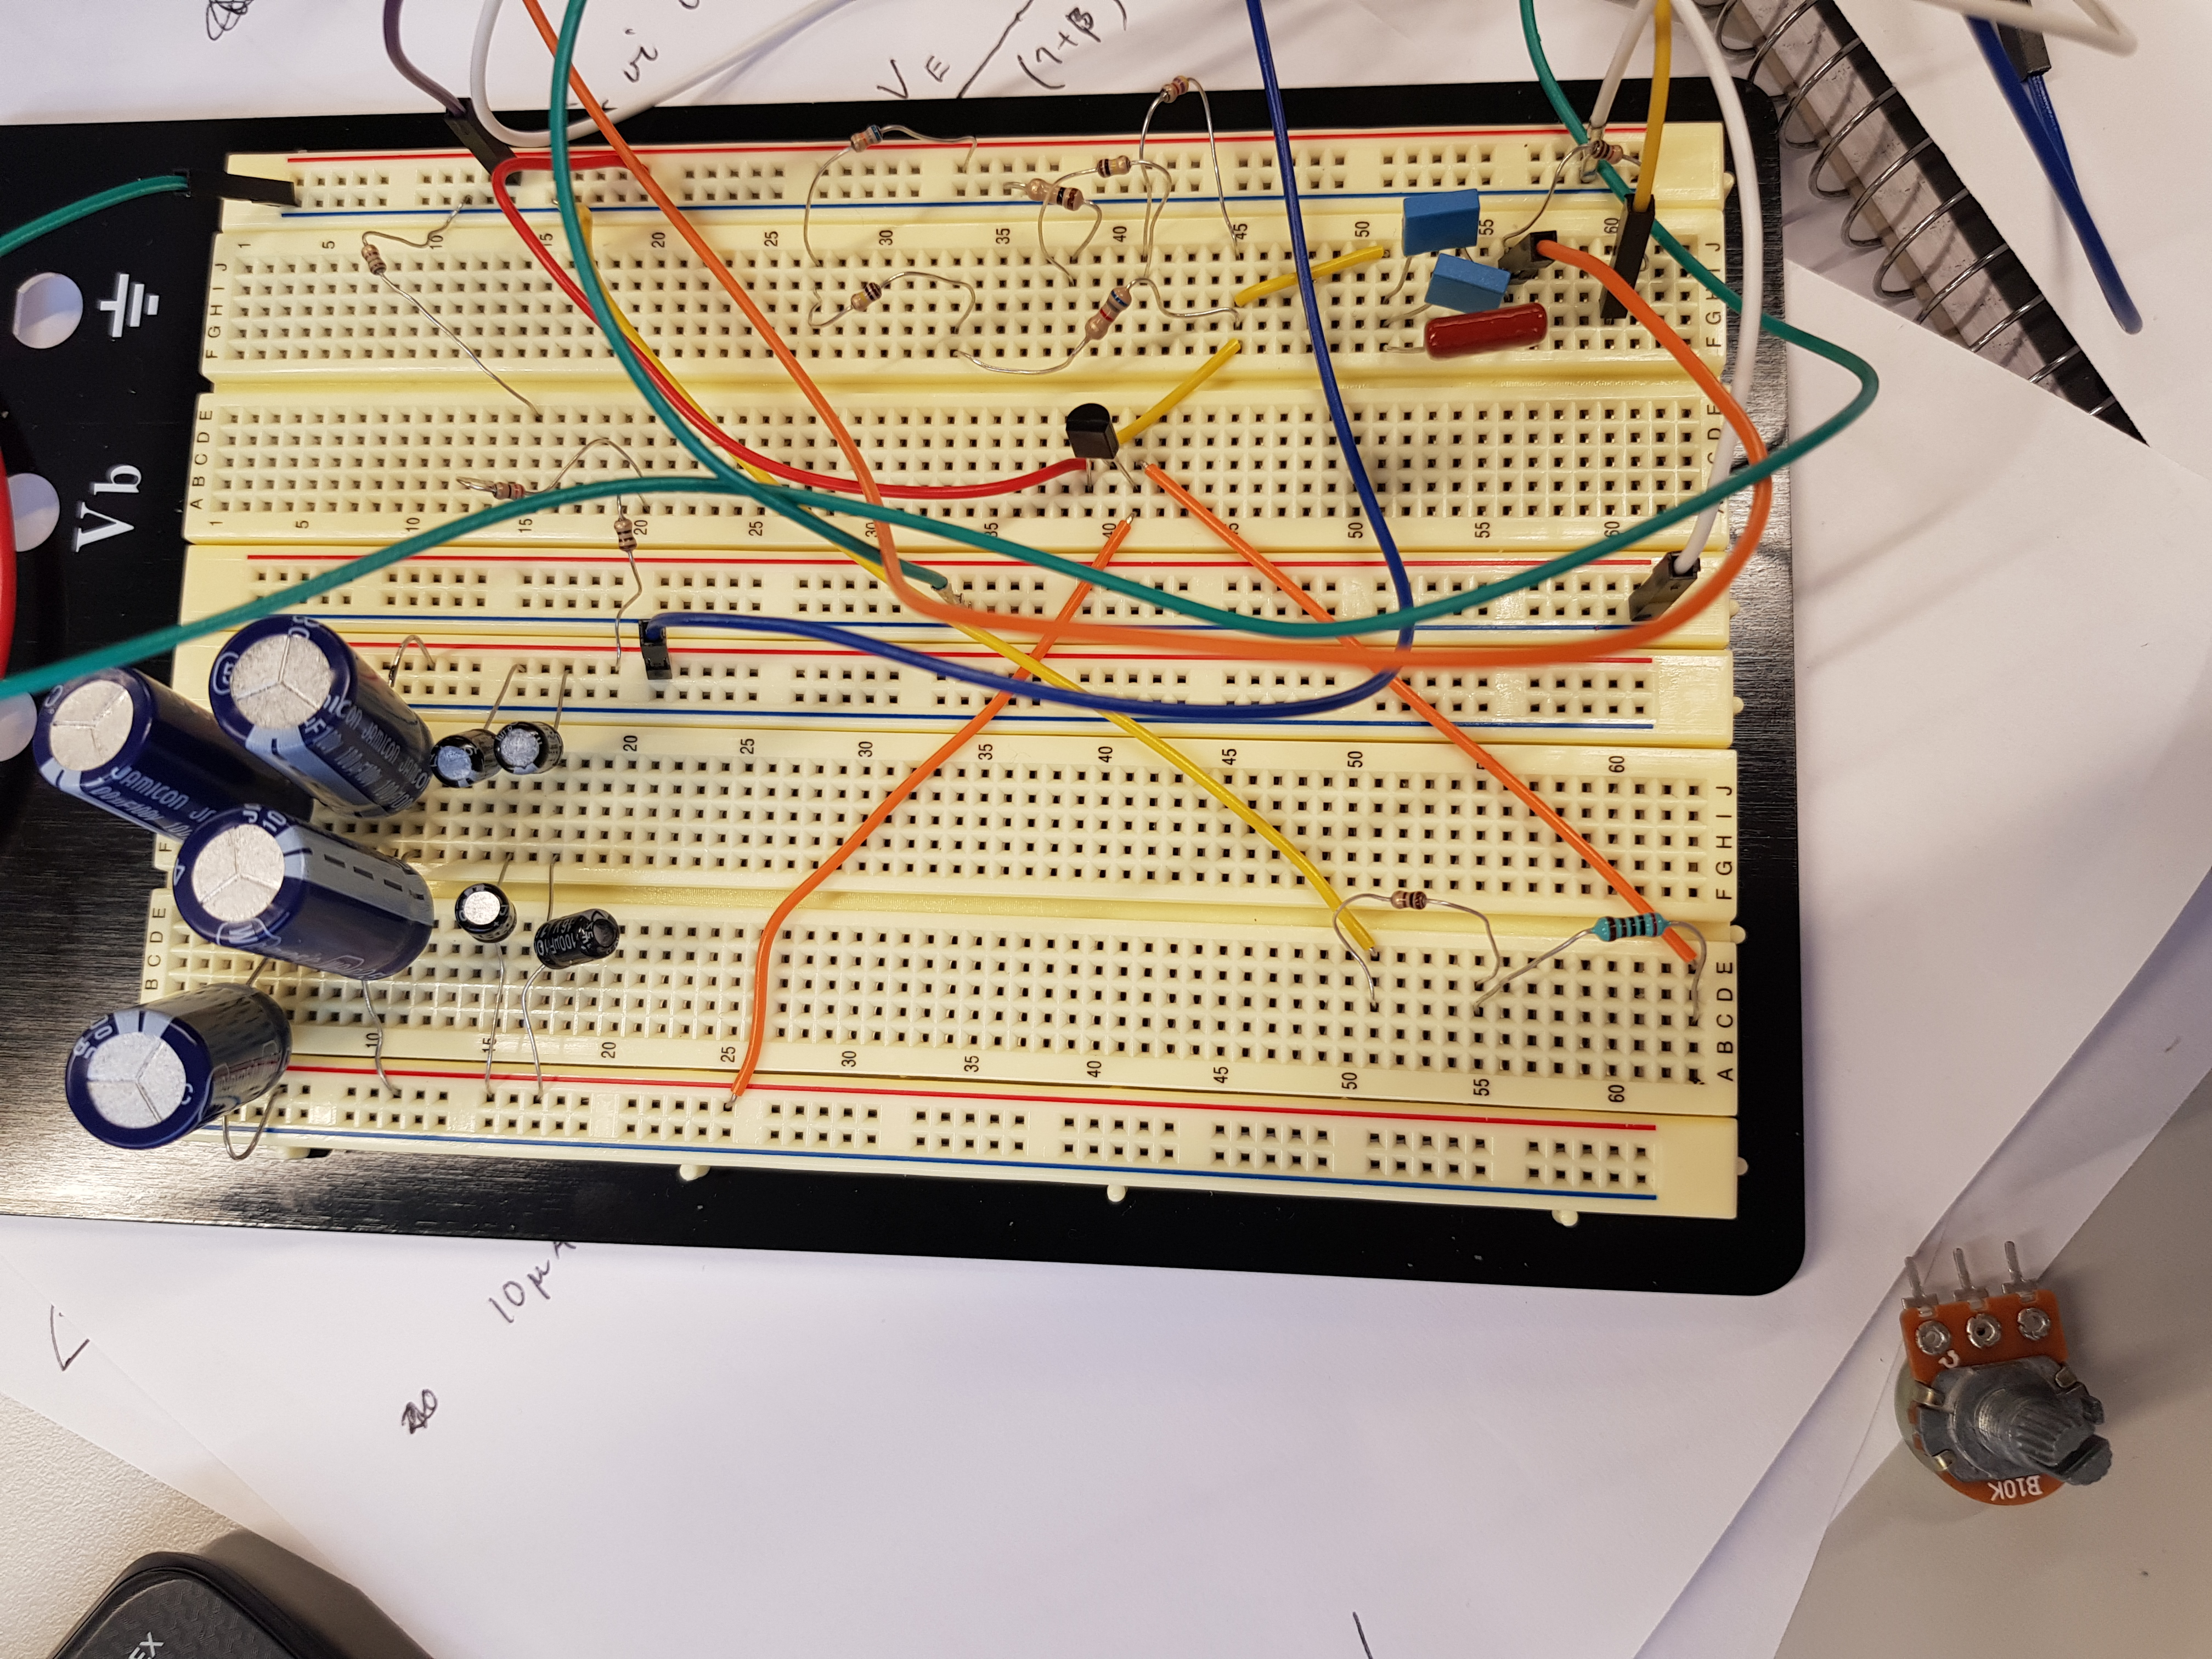
\includegraphics[width=1.0\textwidth]{img/Initial_circuit.jpg}
    \caption{Realisert krets.}
    \label{fig: first circuit}
\end{figure}\\

\newpage

\subsection{Justerer $R_1$}\label{subsec: improved signal}
Ved å minke motstanden på $R_1$ så mye som mulig, så vil $A_v\rightarrow 1$. Ekempelvis gir figur~\ref{fig: improved signal} at $A_v = 0.961$, der $R_1 = 6.67$k$\Omega$.
Det vi oppdager er at amplituden $A_i$ til $v_i(t)$ og $A_o$ til $v_o(t)$ på figuren blir betydelig mindre enn $A_0$. Også forskjellen mellom mellom $A_i$ og $A_o$ blir mindre: \\
\begin{equation}\label{eq: delta A_0}
    \Delta A_0 = A_0 - A_o = 84.2\textrm{mV},
\end{equation}
\begin{equation}\label{eq: delta A_i}
    \Delta A_i = A_i - A_o = 16.3\textrm{mV}.
\end{equation}
\\
Det vi kan gjøre for å forbedre signalet er å utvikle et arbeidspunkt der klippingen så vidt ikke forekommer. Seksjon~\ref{subsec: klipping signal} viser et signal, som nærmer seg klipping. 
\\
\\ En forklaring på hvorfor $|v_i(t)|$ blir mindre, er fordi $V_k = I / R_k$ øker når $Z_i$ minker.

\begin{figure}[htbp]
    \centering
    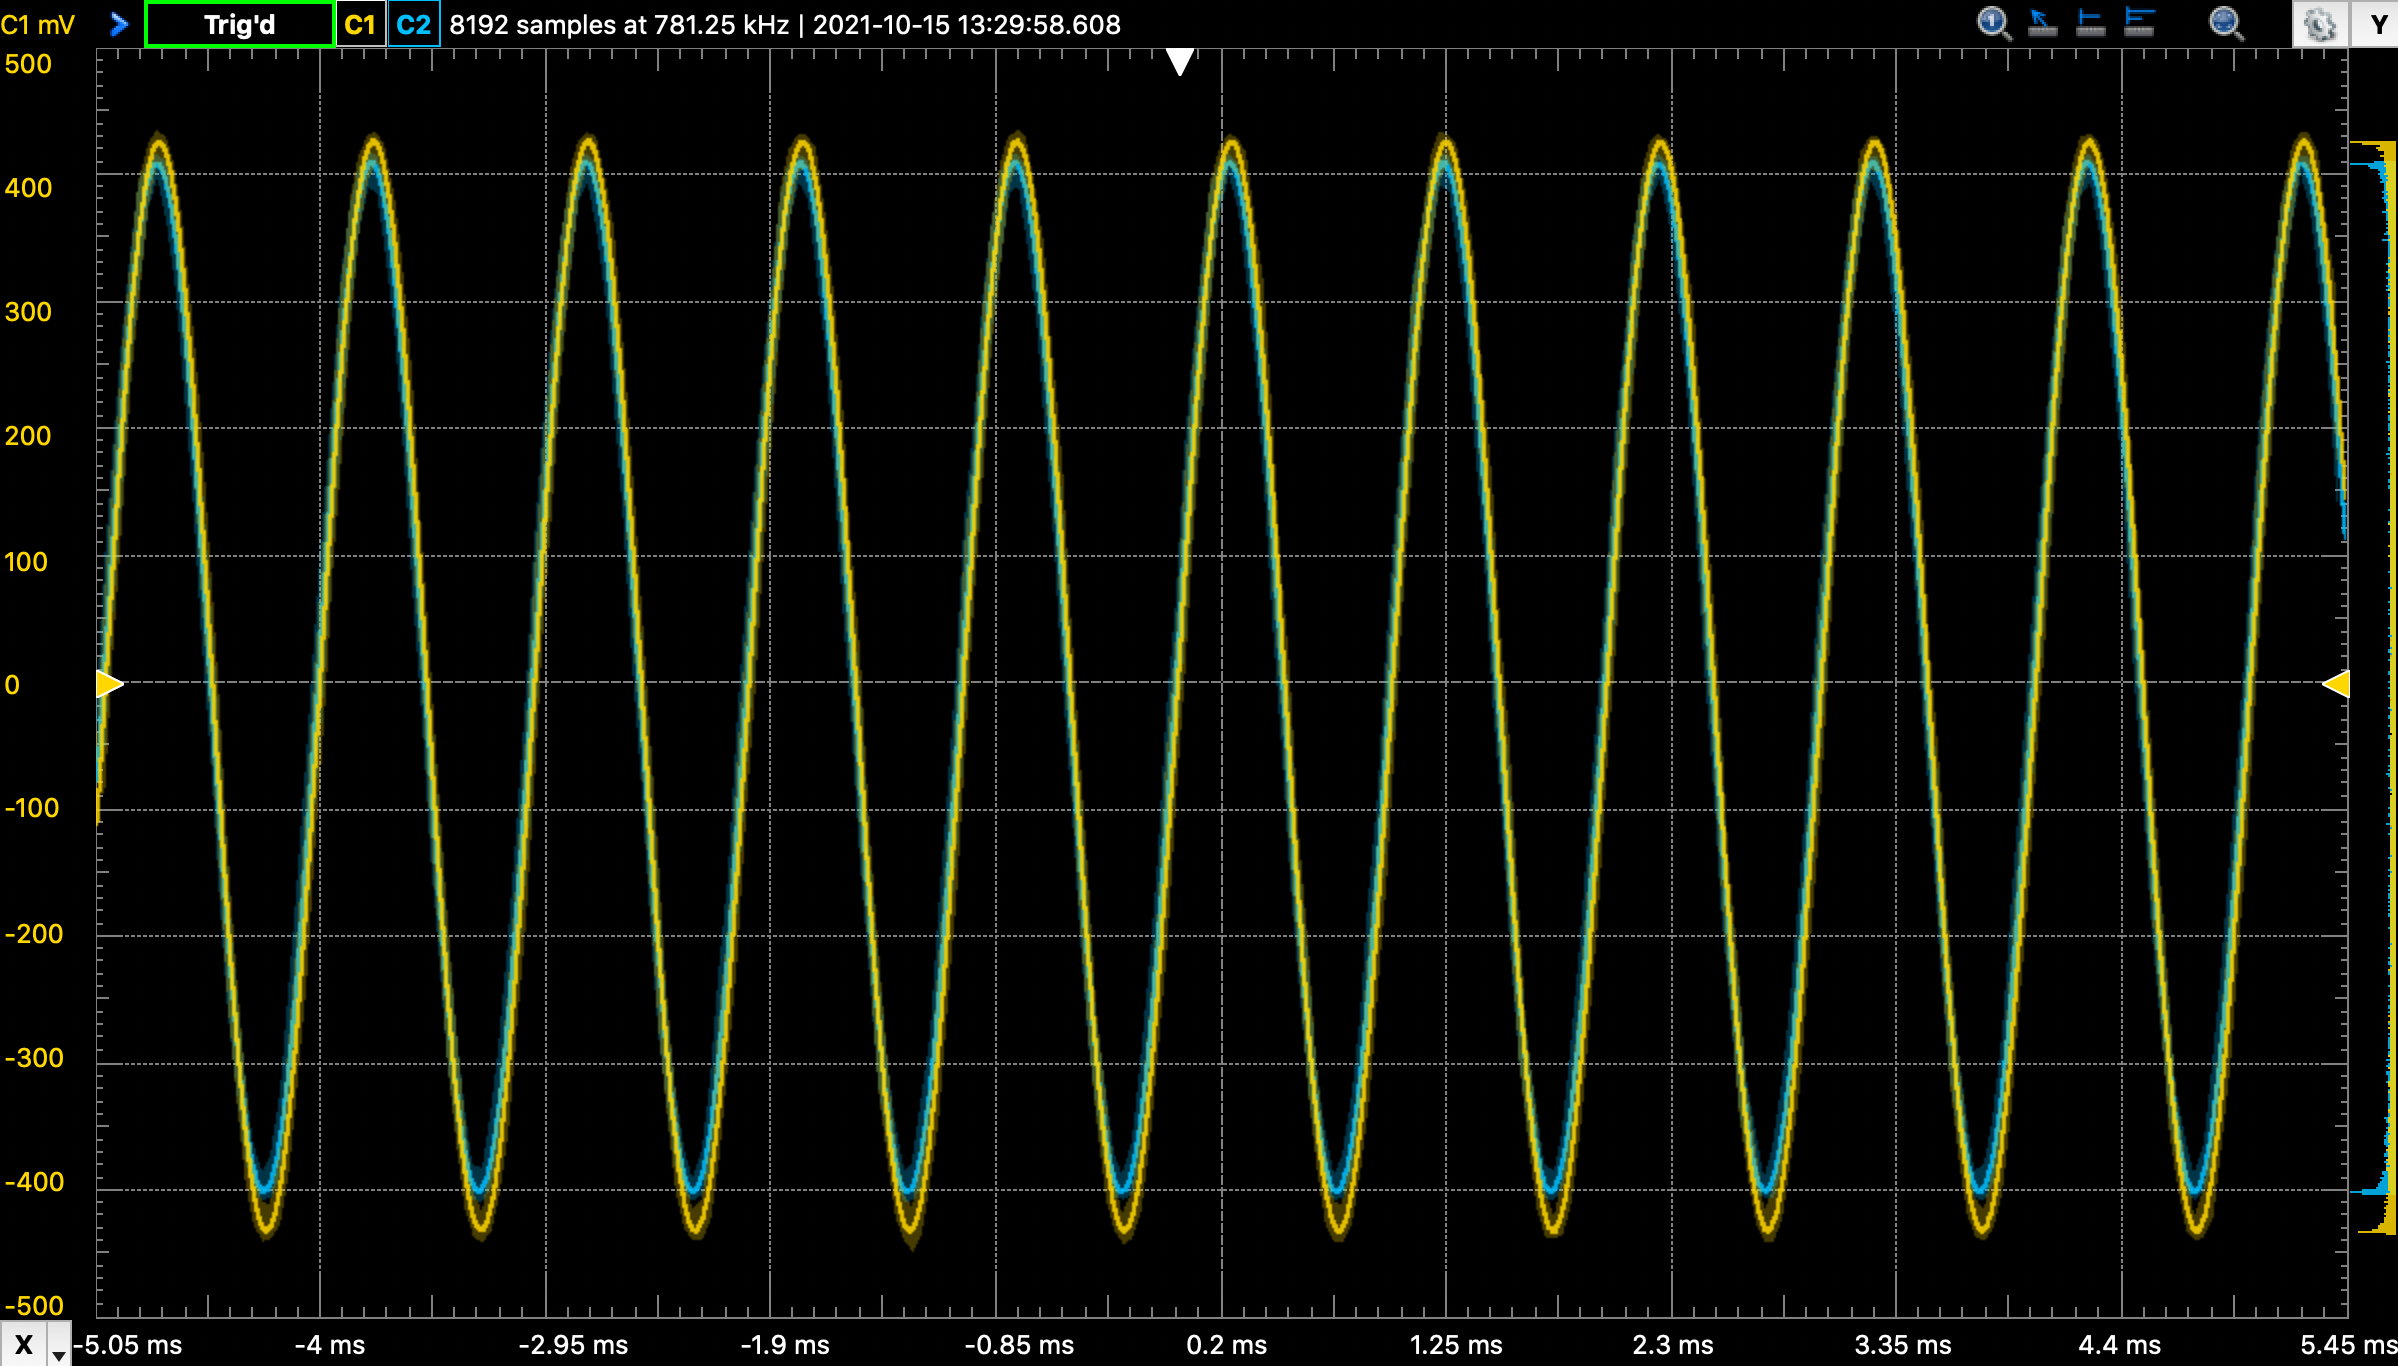
\includegraphics[width=1.0\textwidth]{img/Improved signal.png}
    \caption{Forbedret $A_v$: [V/t], Gul: $v_i(t)$ Turkis: $v_o(t)$.}
    \label{fig: improved signal}
\end{figure}\\
\newpage
\subsection{Rett før klipping}\label{subsec: klipping signal}
For å optimalisere signalet, så ønsker vi å utarbeidet et arbeidspunkt som ligger i grenseland til klipping.
Gjennom prøving og feiling, så vil $R_2 = 66.7$k$\Omega$ gi et området som nærmer seg klipping. Ved å legge på $10$k$\Omega$, så fremkommer tydelig klipping.
Likning~\ref{eq: delta A_0} $\implies \Delta A_0 = 52mV$,
og vi får også en $A_v = 0.931$.
\\\\
Fra seksjon~\ref{subsec: improved signal} til her, så fikk vi nesten en halvering i amplitude-avvik, men det betydde også at signalet mistet mer styrke gjennom bufferen. Så lenge $v_i(t)$ og $v_o(t)$ har lik frekvens og ingen klipping, så er amplitudeavvik ikke kritisk. Det kan eventuelt brukes forsterkere etterpå, dersom det krever nøyaktighet i amplitude.
% R2 = 66.7kohm
% $A_o = 448$mV 
% $A_i = 481$mV
% $A_v =0.931$
\begin{figure}[htbp]
    \centering
    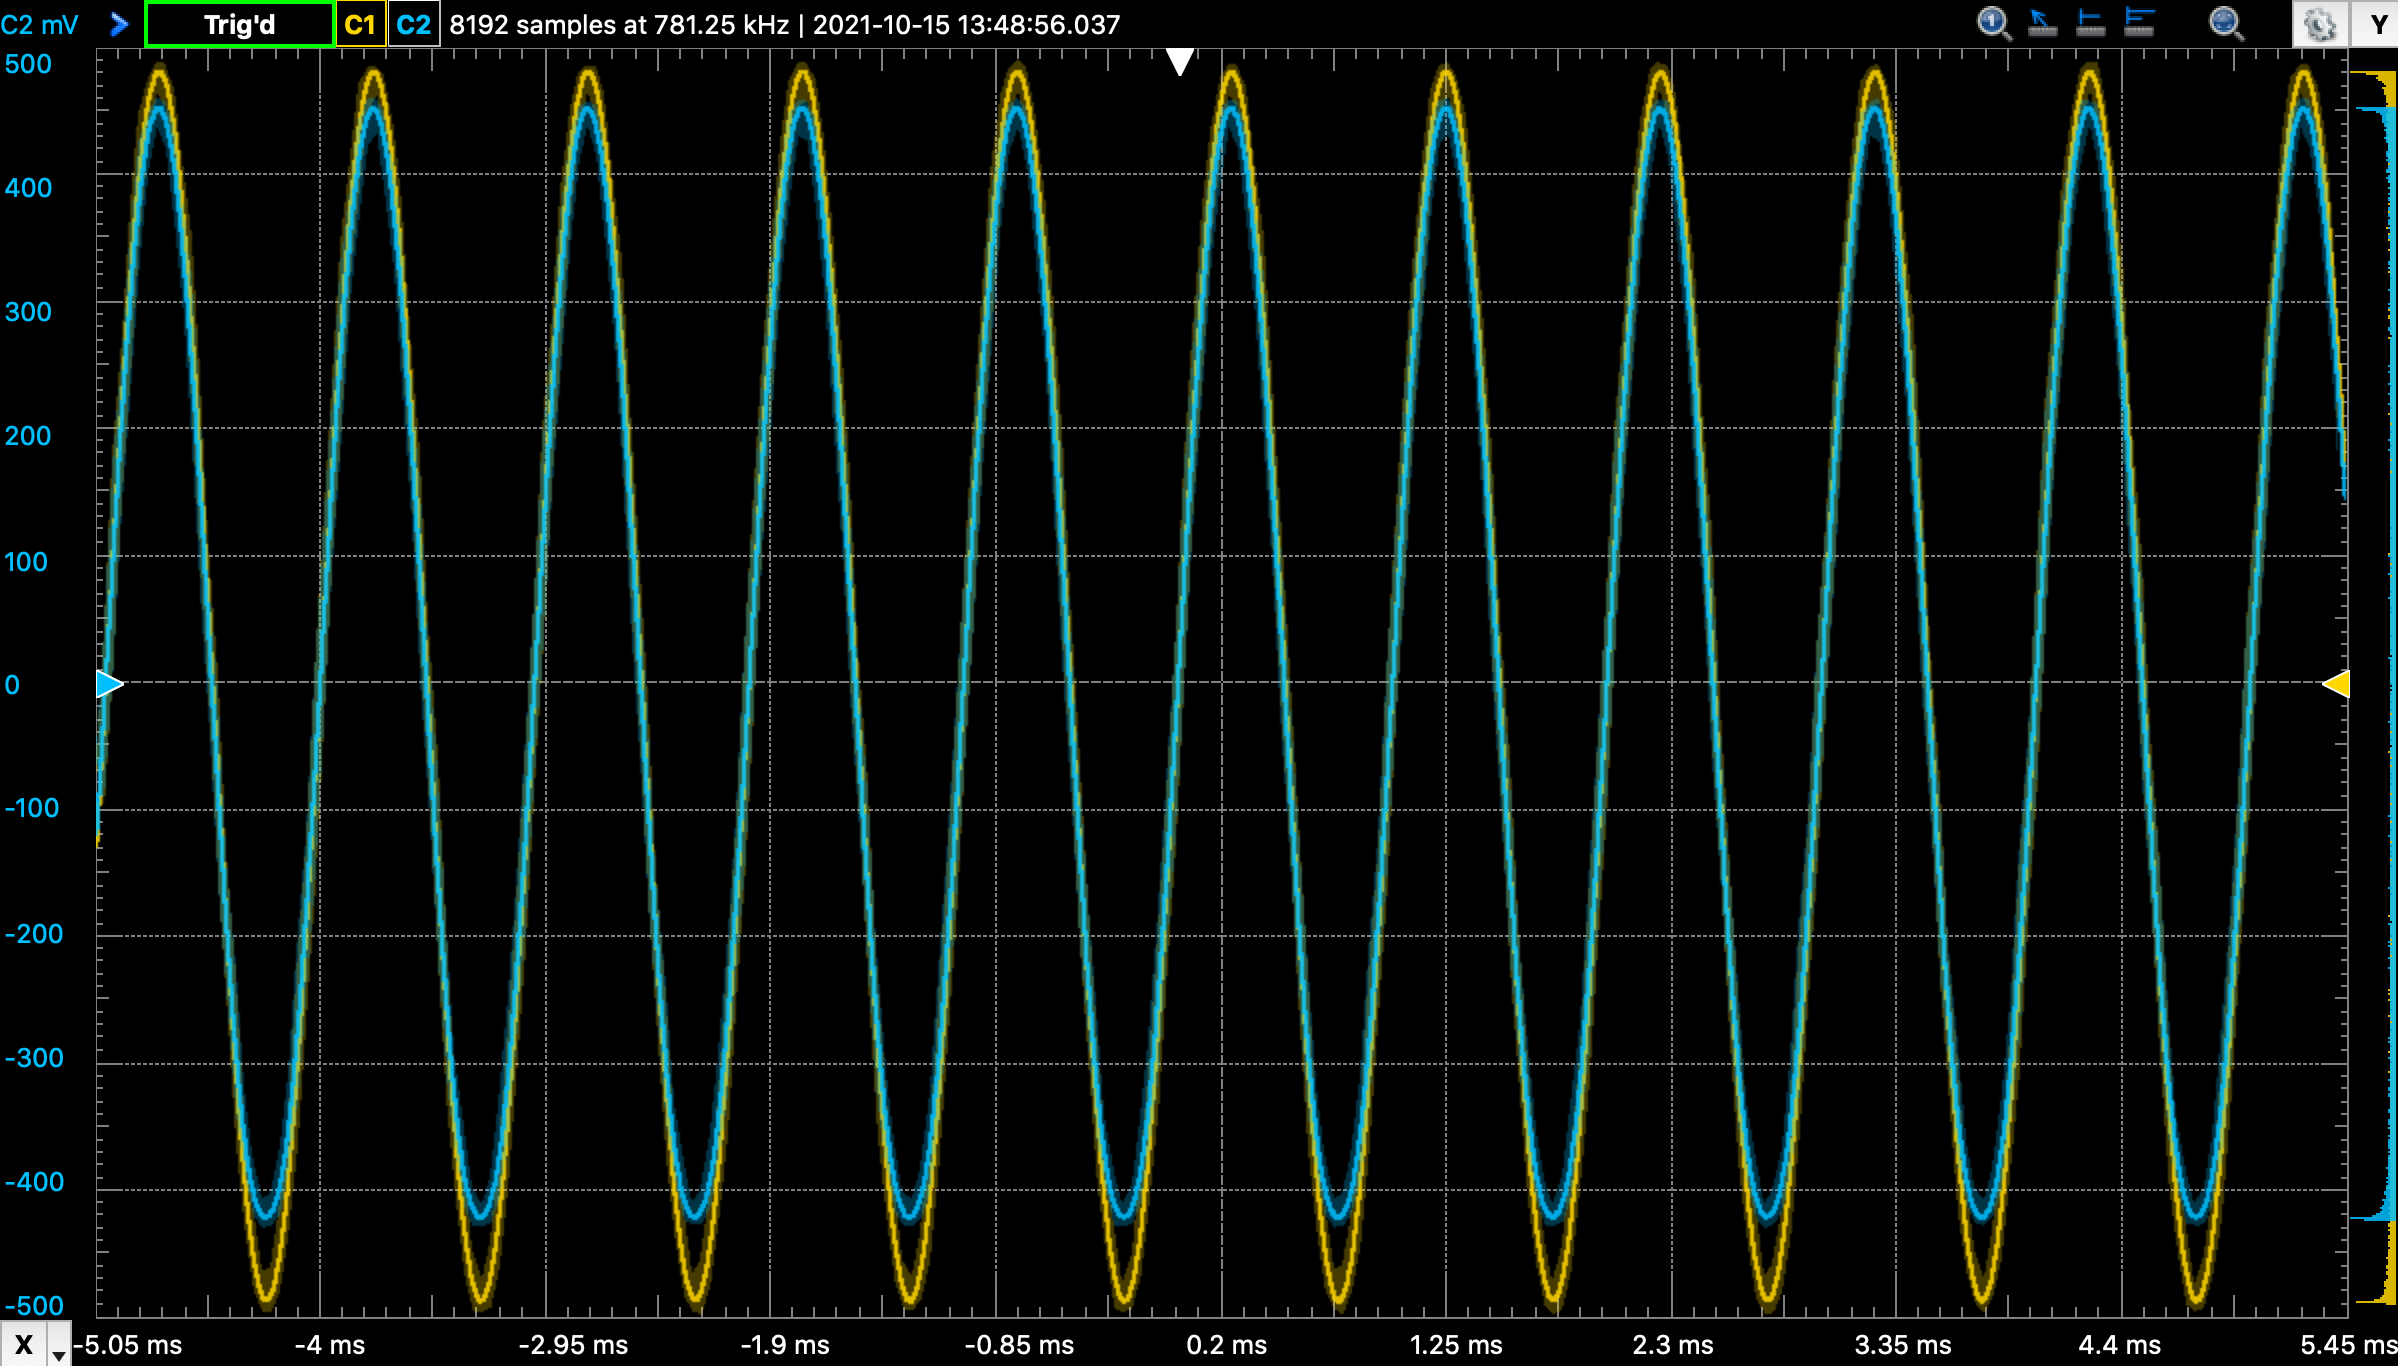
\includegraphics[width=1.0\textwidth]{img/Right before clipping.png}
    \caption{Rett før klipping: [V/t], Gul: $v_i(t)$, Turkis: $v_o(t)$.}
    \label{fig: right before clipping}
\end{figure}\\

Vi kan finne $f_{min}$ til $v_o(t)$ ved å se på frekvensresponsen, som vist ved figur~\ref{fig: knekkfrekvens}.
\newpage
\begin{figure}[htbp]
    \centering
    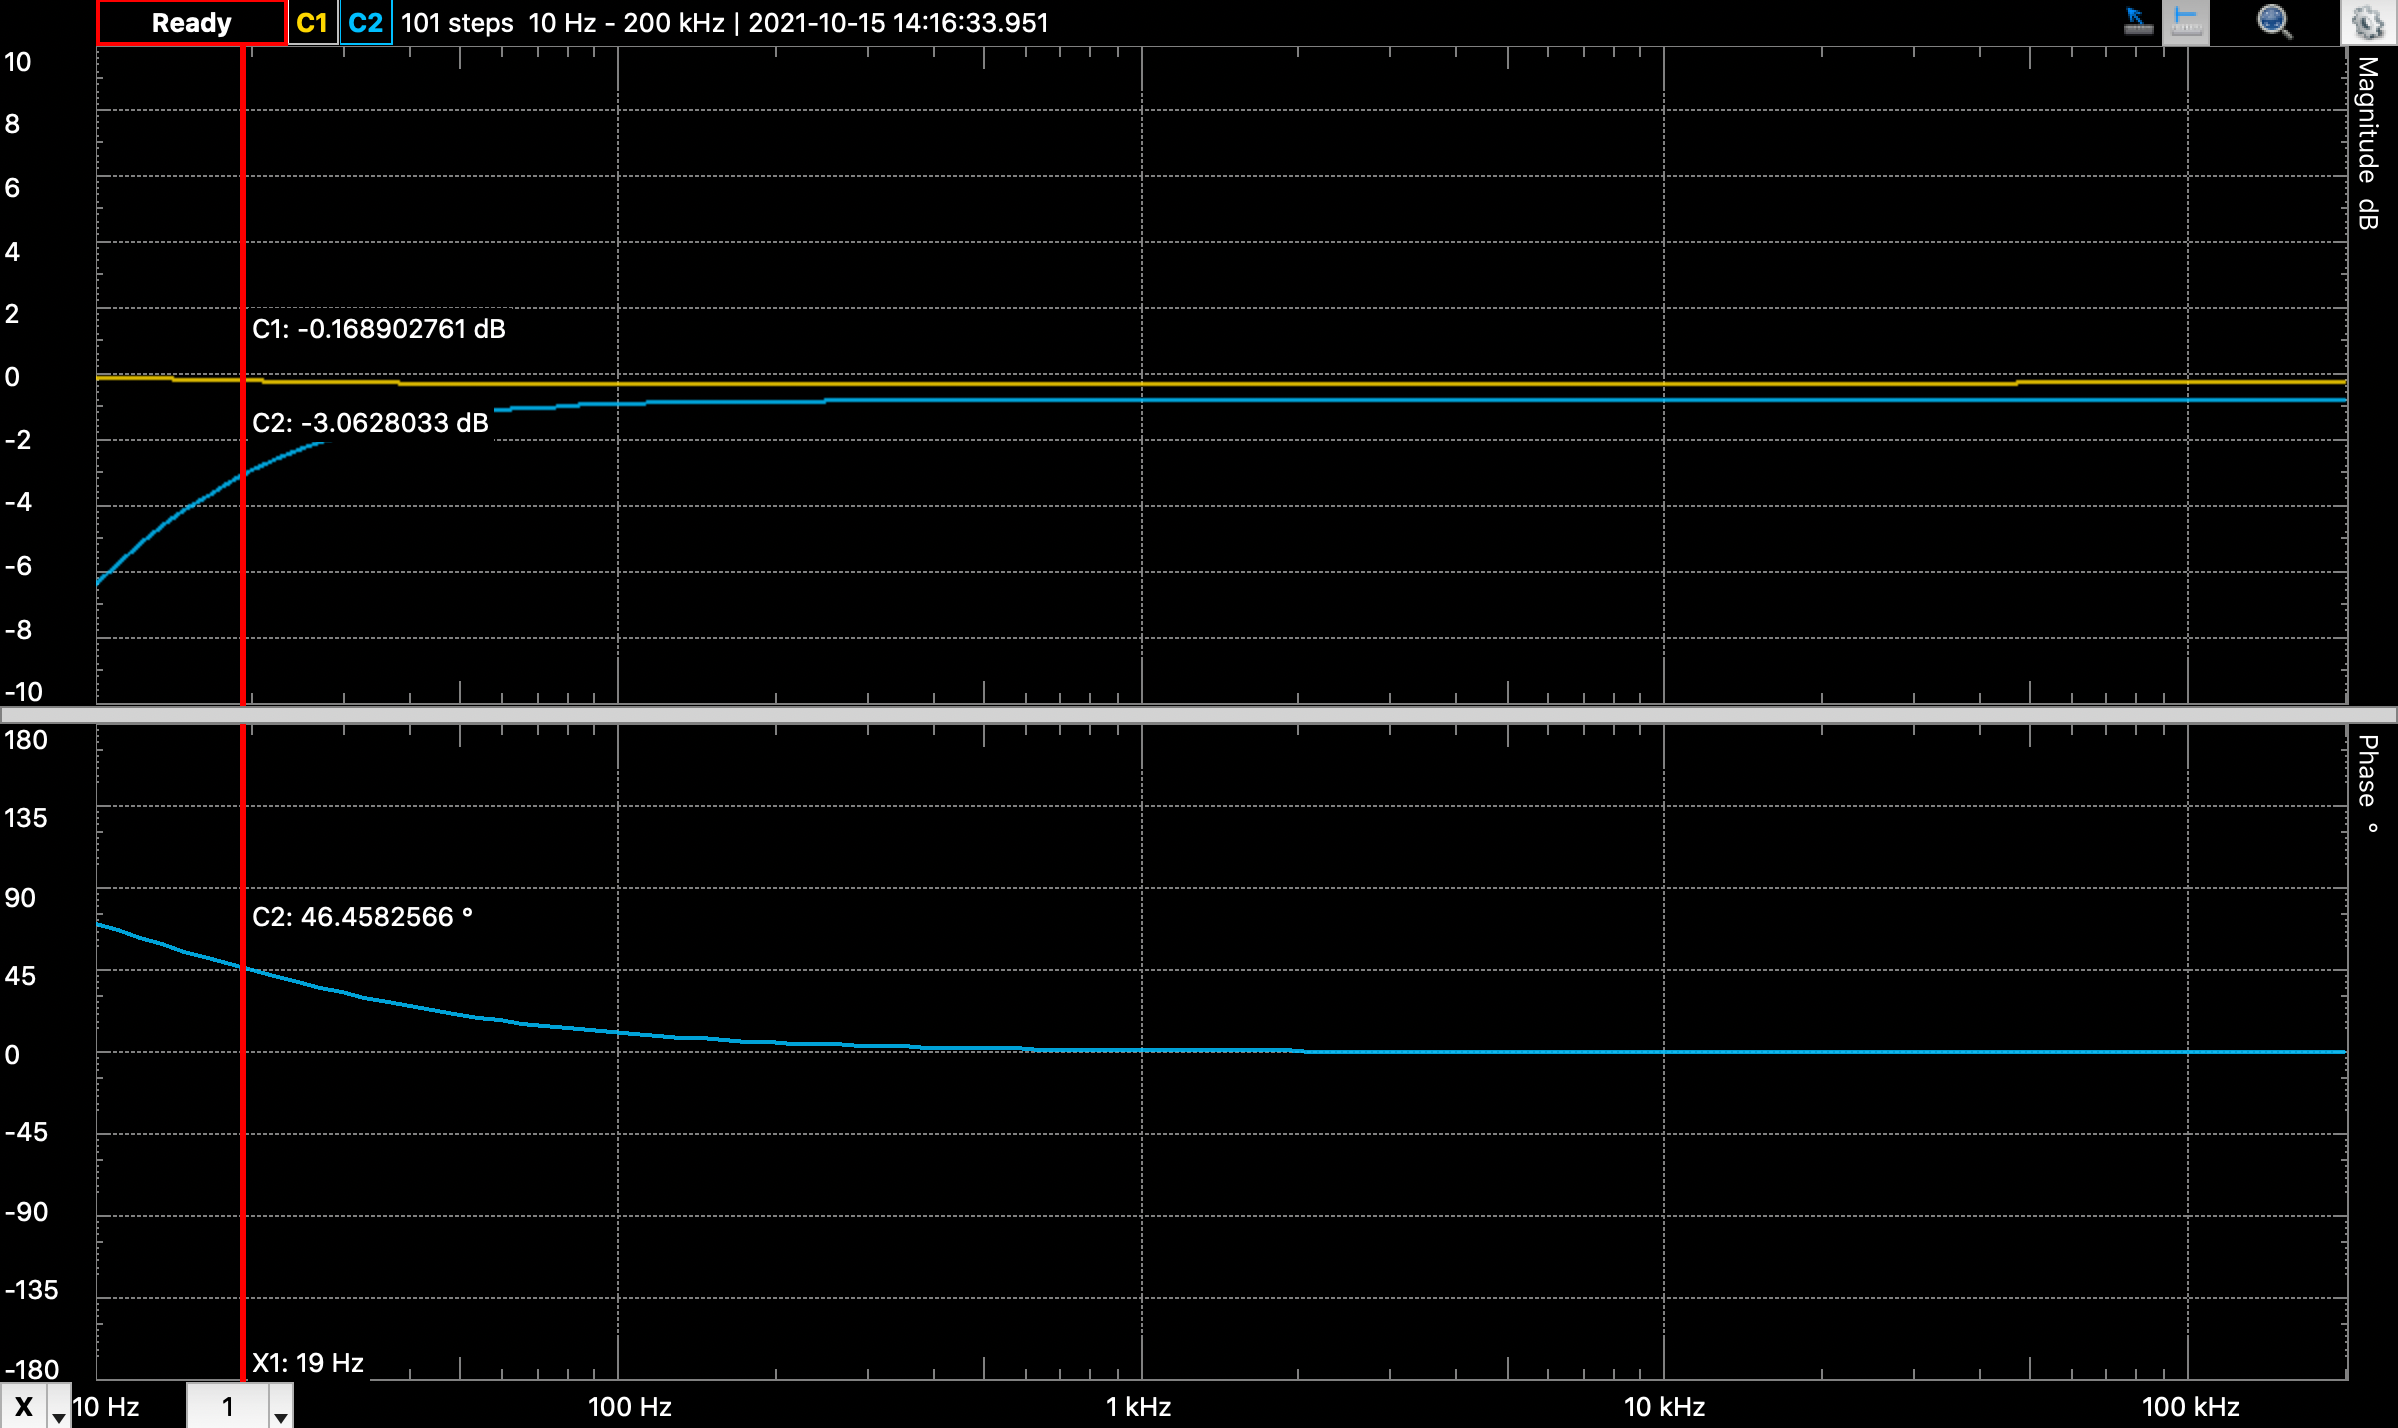
\includegraphics[width=1.0\textwidth]{img/Knekkfrekvens.png}
    \caption{Frekvensresponsen: [dB/Hz], X1: $f_{min}$, Gul: $v_i(t)$, Turkis: $v_o(t)$.}
    \label{fig: knekkfrekvens}
\end{figure}\\
Her ser vi at $f_{min}$ avviker $6$Hz fra den teoretiske nevnt i tabell~\ref{table: variabler}. $C_1$ og $C_2$ er kanskje litt større enn de teoretiske verdier vi regnet ut, men $Z_i$ er betydelig mindre. Det medfører lavere knekkfrekvens, se likning~\ref{eq: C_1}.
\newpage
\section{Konklusjon}
\label{sec:konklusjon}
Det er fullstendig mulig å bruke diskréte komponenter for å lage en buffer. Det er en del endringer fra teoretisk til reell konstruksjon som må gjøres. Blant annet vil $V_B$ ikke ligge der de teoretiske verdiene tilsier. Det andre er at $Z_i$ er vanskelig å få stor nok, slik at motstander (eksempelvis $R_k$), som har et betydelig forhold til $Z_i$ vil påvirke signalets styrke. Utgangsimpedansen og den målte emitter-strømmen oppfører seg derimot som ønsket. 
\\\\
Rett før signalet vil få klipping, så har vi et avvik i amplituden på $10\%$ og avvik på forsterkningen på $6.7\%$. Det kan forbedres ved å bruke ytterligere forsterkere om nødvendig. Signalet som genereres har knekkfrekvens så lav som $19$Hz.
\newpage

\begin{thebibliography}{9}
\bibitem{buffer_article}
    Electrical4U (2021), Artikkel \\
    \emph{Voltage Follower OP Amplifier} \\
    Tilgjengelig ved: \href{https://www.electrical4u.com/voltage-follower/}{https://www.electrical4u.com/voltage-follower/} \\
    (Sist åpnet: 12. Oktober 2021)
\bibitem{BC547B Datasheet}
    Phillips Semiconductor (2004), Datasheet \\
    \emph{BC547B Datasheet} \\
    Tilgjengelig ved: \\
    \href{https://pdf1.alldatasheet.com/datasheet-pdf/view/197561/PHILIPS/BC547B.html}{https://pdf1.alldatasheet.com/datasheet-pdf/view/197561/PHILIPS/BC547B.html} \\
    (Sist åpnet: 13. Oktober 2021)    
\bibitem{Thermal Voltage}
    KurtHeckman (2021), Article \\
    \emph{Thermal Voltage} \\
    Tilgjengelig ved: \href{https://www.vcalc.com/wiki/EmilyB/Thermal+Voltage}{https://www.vcalc.com/wiki/EmilyB/Thermal+Voltage} \\
    (Sist åpnet: 13. Oktober 2021) 
\end{thebibliography}

\newpage
%Bibliografi: Legg til flere elementer ved å legge til flere \bibitem:--------
\phantomsection

\appendix
%Tillegg. Flere tillegg legges til ved å lage flere sections:-----------------


\end{document}